\documentclass[../AnalisiDeiRequisiti.tex]{subfiles}
\begin{document}

\section{Casi d'uso}
Di seguito verranno elencati i casi d'uso ricavati dall'analisi del capitolato C2 e dalle riunioni fatte con \prop.\\
Ogni caso d'uso viene identificato dalla seguente dicitura:
\begin{equation*}
	UC[codice]
\end{equation*}
Dove codice indica il codice univoco con cui verrà indicato ogni caso d'uso.
\newpage
\subsection{Caso d'uso UCG - Visione generale del sistema}
\begin{figure}[!h]
	\centering
	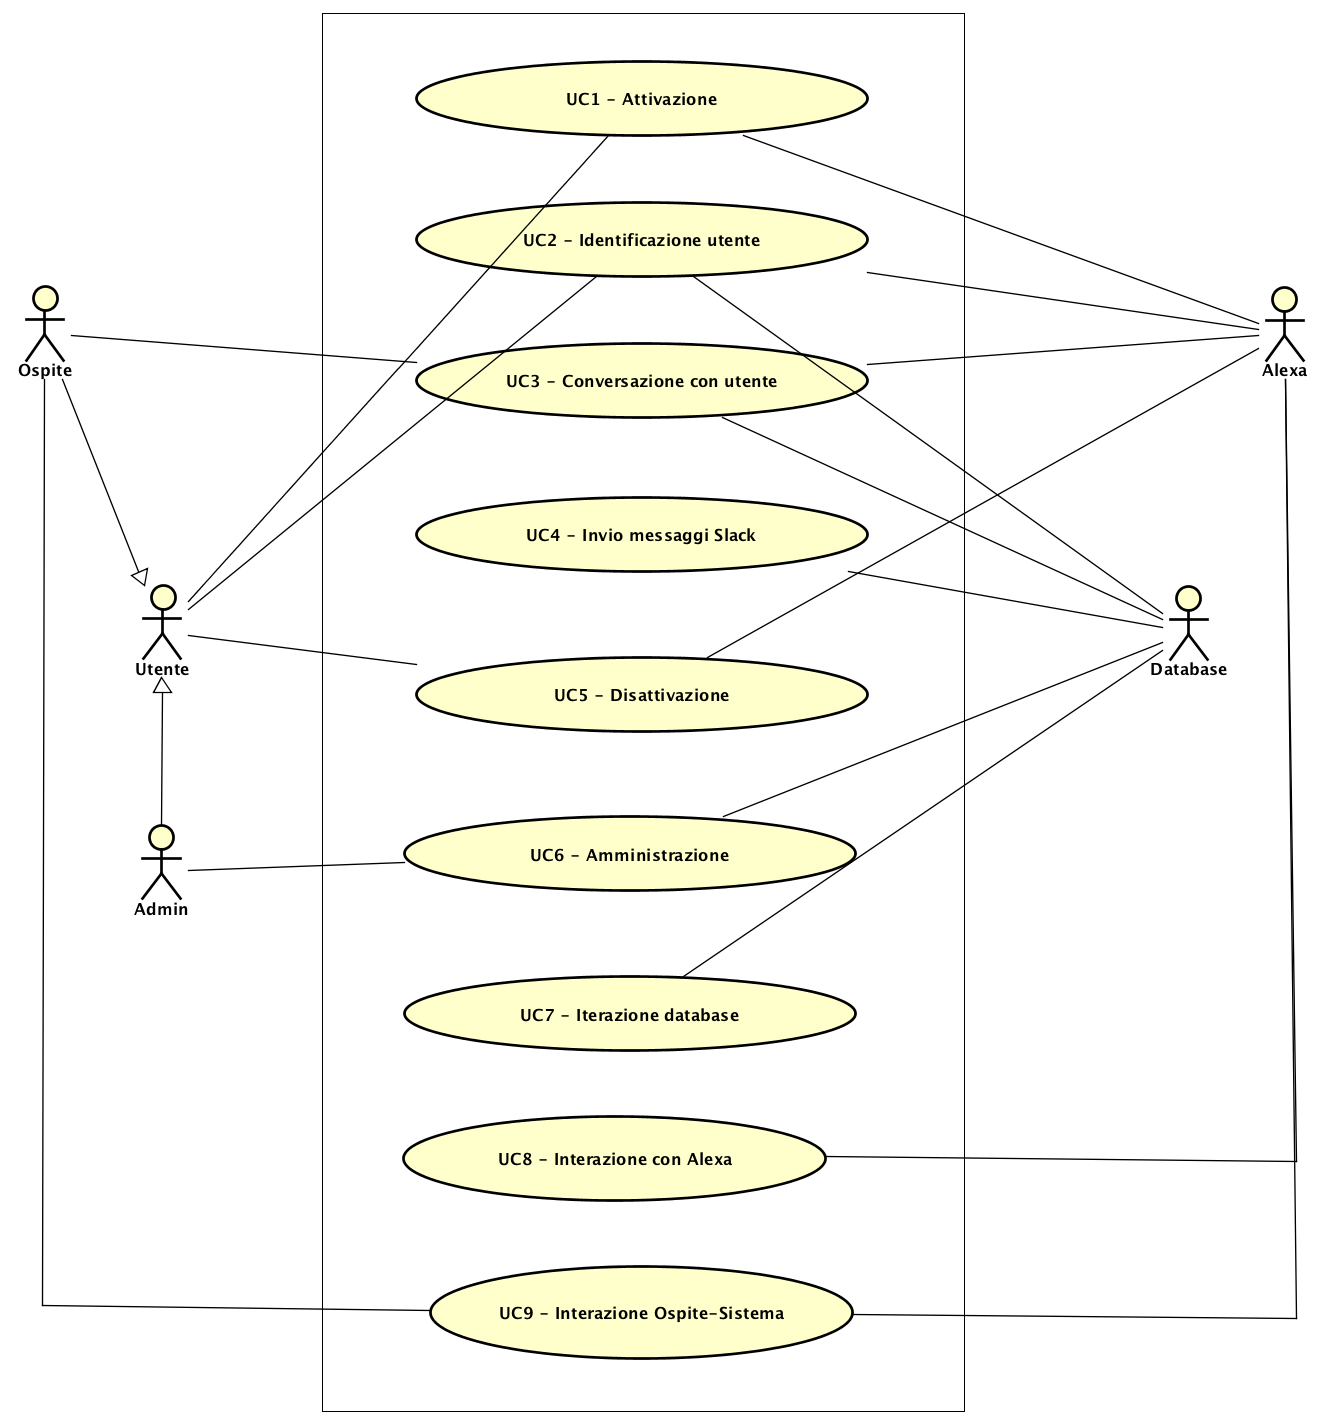
\includegraphics[width=\textwidth]{UseCases/UC_AltoLivello/UC_AltoLivello.png}
	\caption{Caso d'uso UCG - Visione generale del sistema}
\end{figure}	
\begin{itemize} 
\item \textbf{Attori}: utente, ospite, admin, Alexa, database;
\item \textbf{Descrizione}: Un utente può attivare/disattivare il sistema, identificarsi nel sistema. Un ospite, una volta identificato, può conversare con il sistema e quindi interagire con il sistema. Un amministratore, una volta identificato anch'esso, può gestire tutta la parte amministrativa del sistema;
\item \textbf{Precondizione}: Il sistema è correttamente installato nella piattaforma ed esiste un utente, ospite o amministratore, che interagisce col sistema;
\item \textbf{Postcondizione}: Il sistema ha erogato le funzionalità richieste dall'utente. 
\end{itemize} 
\newpage
\subsection{UC1 - Attivazione comunicazione AV}
\begin{figure}[!h]
	\centering
	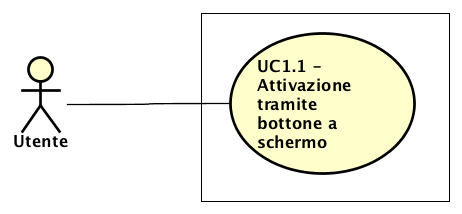
\includegraphics[width=\textwidth]{UseCases/UC1-Attivazione/UC1.png}
	\caption{UC1 - Attivazione comunicazione AV}
\end{figure}	
\label{sssec:UC1} 
\begin{itemize} 
\item \textbf{Attori}: utente;
\item \textbf{Descrizione}: attivazione della comunicazione con l'utente e inizio della conversazione;
\item \textbf{Precondizione}: l'utente attiva l'AV;
\item \textbf{Postcondizione}: UC2.
\begin{itemize}
	\item Attivazione tramite bottone a schermo (UC1.1).
\end{itemize}
\end{itemize} 
\subsection{UC1.1 - Attivazione tramite bottone a schermo} 
\label{sssec:UC1.1} 
\begin{itemize} 
\item \textbf{Attori}: ospite;
\item \textbf{Descrizione}: l'utente preme un pulsante sullo schermo e l'AV viene attivato;
\item \textbf{Precondizione}: l'utente preme un pulsante sull'interfaccia;
\item \textbf{Postcondizione}: l'AV viene attivato;
\item \textbf{Scenario principale}: l'AV è in attesa di attivazione. L'ospite lo attiva premendo un bottone a schermo.\end{itemize} 
\newpage
\subsection{UC2 - Identificazione dell'utente}
\begin{figure}[!h]
	\centering
	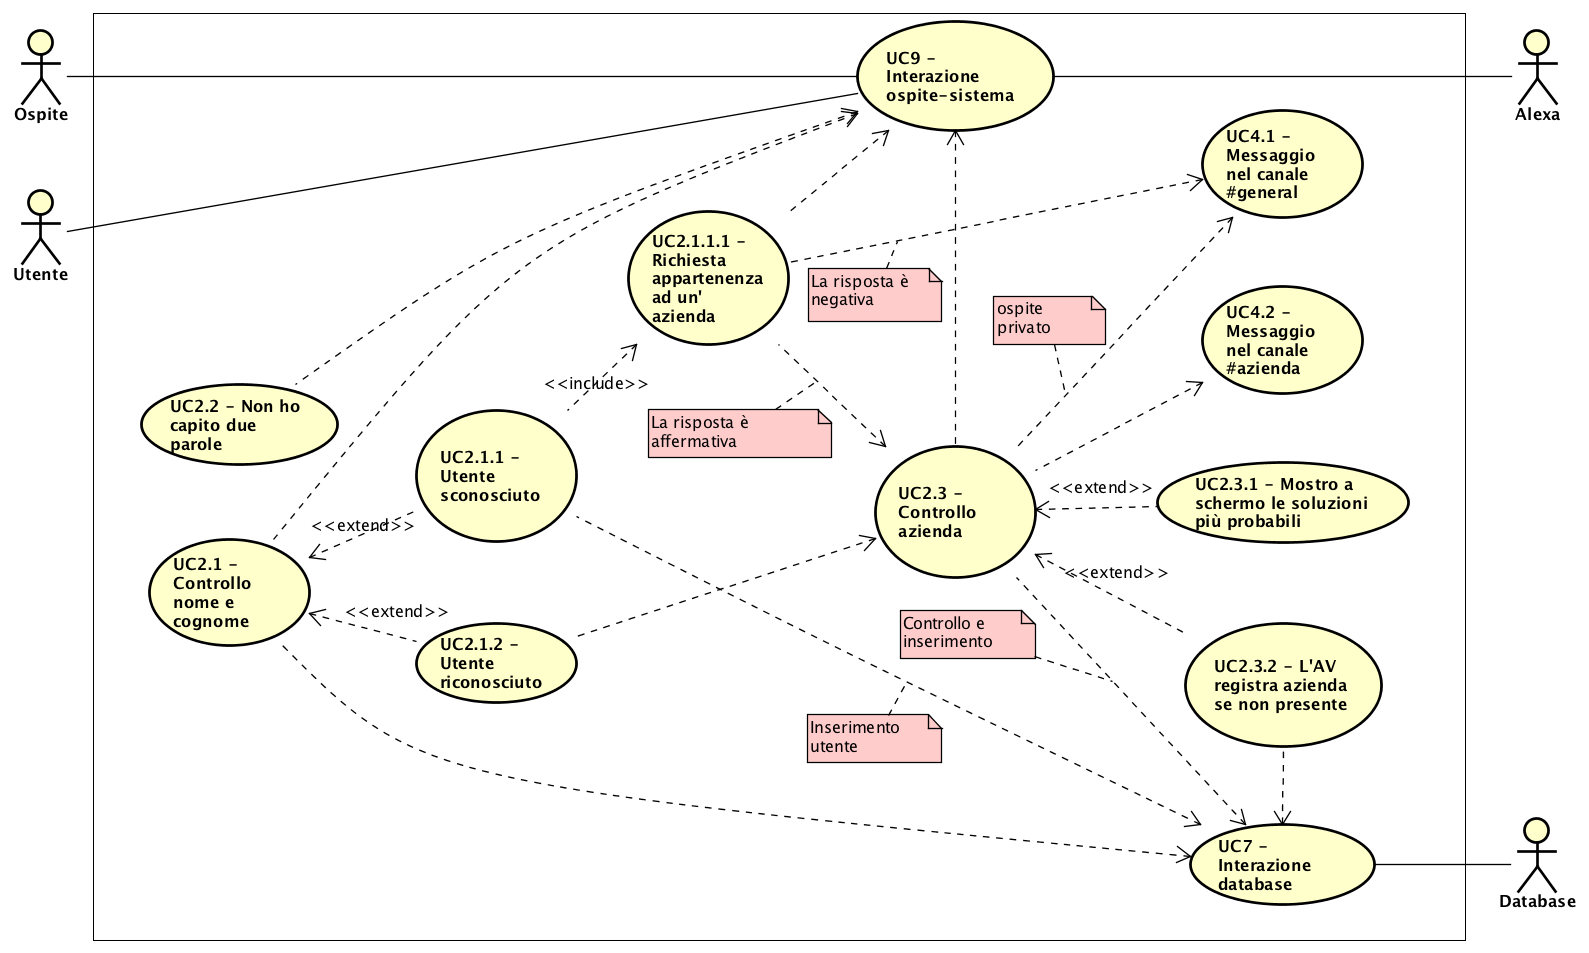
\includegraphics[width=\textwidth]{UseCases/UC2-Identificazione/UC2.png}
	\caption{UC2 - Identificazione dell'utente}
\end{figure}
\label{sssec:UC2} 
\begin{itemize} 
\item \textbf{Attori}: Alexa, ospite.
\item \textbf{Descrizione}: l'AV chiede all'utente il proprio nome e cognome;
\item \textbf{Precondizione}: l'utente pronuncia i propri nome e cognome;
\item \textbf{Postcondizione}: l'AV ottiene il nome e il cognome dell'utente.
\begin{enumerate}
	\item AV non riconosce l'input vocale (UC2.2);\item Controllo azienda (UC2.3). 
 \end{enumerate}
\item \textbf{Scenari alternativi}: l'AV chiede il nome e il cognome dell'utente e l'utente non risponde o Alexa non riesce a capire quello che dice.
\item \textbf{Estensioni}:\begin{itemize}\item controllo nome e cognome (UC2.1).\end{itemize}
\end{itemize} 
\subsection{UC2.1 - Controllo nome e cognome} 
\label{sssec:UC2.1} 
\begin{itemize} 
\item \textbf{Attori}: database;
\item \textbf{Descrizione}: vengono controllati se nome e cognome  appartengono ad un utente nel DB;
\item \textbf{Precondizione}: l'AV ha compreso nome e cognome;
\item \textbf{Postcondizione}: esito della ricerca basato su nome e cognome;
\item \textbf{Scenari alternativi}: utente sconosciuto. Si procede alla domanda di appartenenza ad un'azienda o meno;
\item \textbf{Estensioni}:\begin{itemize}\item utente sconosciuto (UC2.1.1);\item utente riconosciuto (UC2.1.2).\end{itemize}
\end{itemize} 
\subsection{UC2.1.1 - Utente sconosciuto} 
\label{sssec:UC2.1.1} 
\begin{itemize} 
\item \textbf{Attori}: database;
\item \textbf{Descrizione}: il nome e il cognome non si riferiscono a una persona che ha già visitato Zero12;
\item \textbf{Precondizione}: ci sono nome e cognome;
\item \textbf{Postcondizione}: viene chiesto se lavora per un'azienda;
\item \textbf{Scenario principale}: \begin{enumerate}\item richiesta appartenenza ad un'azienda (UC2.1.1.1). 
 \end{enumerate}
\item \textbf{Scenari alternativi}: il nome e il cognome hanno corrispondenza nel DB.
\end{itemize} 
\subsection{UC2.1.1.1 - Richiesta appartenenza ad un'azienda} 
\label{sssec:UC2.1.1.1} 
\begin{itemize} 
\item \textbf{Attori}: Alexa;
\item \textbf{Descrizione}: viene richiesto all'ospite se lavora per un'azienda;
\item \textbf{Precondizione}: l'ospite non era mai stato in zero12 (non era presente nel DB);
\item \textbf{Postcondizione}: si conosce l'appartenenza o meno dell'ospite ad un'azienda;
\item \textbf{Scenario principale}: viene richiesto all'utente se appartiene ad un'azienda o meno. In caso positivo si procede alla richiesta del nome dell'azienda.\end{itemize} 
\subsection{UC2.1.2 - Utente riconosciuto} 
\label{sssec:UC2.1.2} 
\begin{itemize} 
\item \textbf{Attori}: database;
\item \textbf{Descrizione}: l'utente cercato è presente nel database;
\item \textbf{Precondizione}: nel database c'è una corrispondenza con l'utente cercato;
\item \textbf{Postcondizione}: l'utente "generico" ora è identificato e diventa "ospite";
\item \textbf{Scenario principale}: l'utente viene identificato e diventa ospite e successivamente verrà richiesta richiesta la conferma dell'azienda.\end{itemize} 
\subsection{UC2.2 - AV non riconosce l'input vocale} 
\label{sssec:UC2.2} 
\begin{itemize} 
\item \textbf{Attori}: Alexa;
\item \textbf{Descrizione}: AV non riconosce l'input vocale di almeno due parole;
\item \textbf{Precondizione}: l'ospite ha risposto all'AV e l'AV ha decifrato il testo;
\item \textbf{Postcondizione}: l'AV richiede nuovamente nome e cognome;
\item \textbf{Scenario principale}: l'ospite risponde all'AV e l'AV non ne riconosce nome e cognome.\end{itemize} 
\subsection{UC2.3 - Controllo azienda} 
\label{sssec:UC2.3} 
\begin{itemize} 
\item \textbf{Attori}: Alexa, database, ospite;
\item \textbf{Descrizione}: rilevo l'azienda dell'ospite e registro la sua visita;
\item \textbf{Precondizione}: l'ospite è stato identificato;
\item \textbf{Postcondizione}: la visita dell'ospite viene registrata;
\item \textbf{Scenario principale}: \begin{enumerate}\item mostra a schermo le soluzioni più probabili (UC2.3.1). 
 \end{enumerate}
\item \textbf{Scenari alternativi}: se l'ospite lavora per un'azienda e questa non è nel DB viene aggiunta (UC2.3.2).
Viene registrata la visita dell'ospite nel DB.
\item \textbf{Estensioni}:\begin{itemize}\item l'AV registra azienda se non presente (UC2.3.2).\end{itemize}
\end{itemize} 
\subsection{UC2.3.1 - Mostra a schermo le soluzioni più probabili} 
\label{sssec:UC2.3.1} 
\begin{itemize} 
\item \textbf{Attori}: database, ospite;
\item \textbf{Descrizione}: viene mostrato allo schermo una lista delle probabili aziende per cui l'ospite potrebbe lavorare;
\item \textbf{Precondizione}: l'ospite è identificato e lavora per un'azienda;
\item \textbf{Postcondizione}: viene mostrato allo schermo una lista delle probabili aziende per cui l'ospite potrebbe lavorare;
\item \textbf{Scenario principale}: viene mostrato allo schermo una lista delle probabili aziende per cui l'ospite potrebbe lavorare. Anche nessuna se l'ospite è un privato.\end{itemize} 
\subsection{UC2.3.2 - L'AV registra azienda se non presente} 
\label{sssec:UC2.3.2} 
\begin{itemize} 
\item \textbf{Attori}: Alexa, database;
\item \textbf{Descrizione}: se l'ospite viene per conto di un'azienda non presente nel DB, questa viene aggiunta;
\item \textbf{Precondizione}: l'ospite è identificato e viene per conto di un'azienda non presente nel DB;
\item \textbf{Postcondizione}: l'azienda dell'ospite viene aggiunta al DB;
\item \textbf{Scenario principale}: se l'ospite viene per conto di un'azienda non presente nel DB, questa viene aggiunta (Interazione con database).\end{itemize} 
\newpage
\subsection{UC3 - Conversazione con ospite}
\begin{figure}[!h]
	\centering
	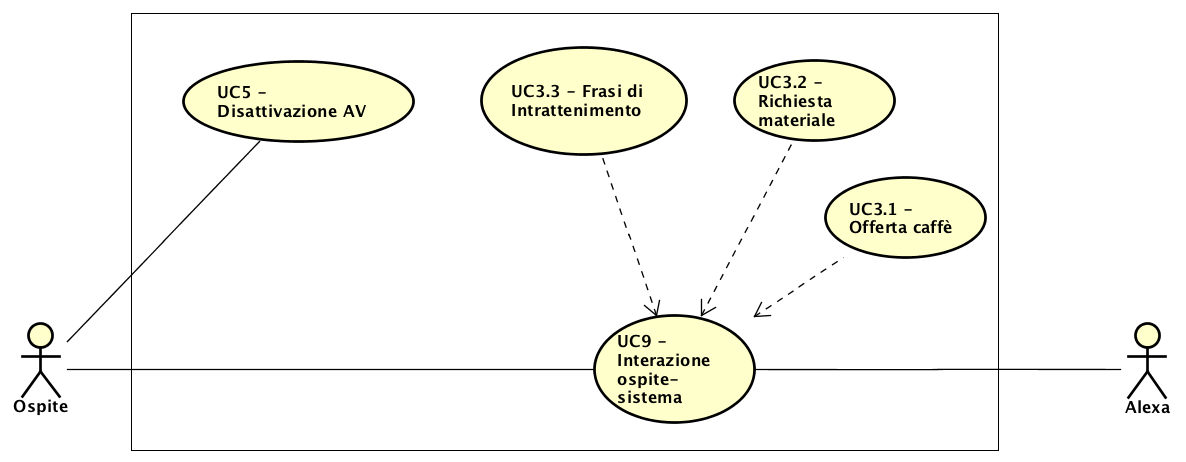
\includegraphics[width=\textwidth]{UseCases/UC3-Conversazione/UC3.png}
	\caption{UC3 - Conversazione con ospite}
\end{figure}
\label{sssec:UC3}
\begin{itemize} 
\item \textbf{Attori}: Alexa, database, ospite;
\item \textbf{Descrizione}: conversazione con ospite;
\item \textbf{Precondizione}: ospite identificato nel caso d'uso UC2;
\item \textbf{Postcondizione}: l'ospite ha concluso tutte le interazioni possibili con il sistema;
\item \textbf{Estensioni}:\begin{itemize}\item offerta caffè (UC3.1);\item richiesta materiale (UC3.2);\item frasi di intrattenimento (UC3.3).\end{itemize}
\end{itemize} 
\subsection{UC3.1 - Offerta caffè} 
\label{sssec:UC3.1} 
\begin{itemize} 
\item \textbf{Attori}: Alexa, database, ospite, Slack;
\item \textbf{Descrizione}: viene offerto il caffè all'ospite;
\item \textbf{Precondizione}: utente identificato;
\item \textbf{Postcondizione}: messaggio Slack di conferma del caffè;
\item \textbf{Scenario principale}: 1)viene chiesto all'ospite se vuole il caffè
2)viene inviata al canale Slack la risposta.\end{itemize} 
\subsection{UC3.2 - Richiesta materiale} 
\label{sssec:UC3.2} 
\begin{itemize} 
\item \textbf{Attori}: Alexa, database, ospite, Slack;
\item \textbf{Descrizione}: offerta del materiale di materiale per l'incontro;
\item \textbf{Precondizione}: utente identificato;
\item \textbf{Postcondizione}: messaggio Slack;
\item \textbf{Scenario principale}: 1)il sistema richiede la necessità di meteriale all'ospite
2)invio risposta con un messaggio Slack.\end{itemize} 
\subsection{UC3.3 - Frasi di intrattenimento} 
\label{sssec:UC3.3} 
\begin{itemize} 
\item \textbf{Attori}: Alexa, database, ospite;
\item \textbf{Descrizione}: uso di frasi di intrattenimento per far trascorrere il tempo all'ospite in attesa;
\item \textbf{Precondizione}: utente identificato;
\item \textbf{Postcondizione}: fine dell'interazione;
\item \textbf{Scenario principale}: 
	\begin{enumerate}
		\item frase di intrattenimento;
		\item viene richiesto se si vuole ascoltare un'ulteriore frase;
		\item iterazione di 1) e 2);
		\item chiusura della sessione.
	\end{enumerate}
\end{itemize} 
\newpage
\subsection{UC4 - Invio messaggio} 
\begin{figure}[!h]
	\centering
	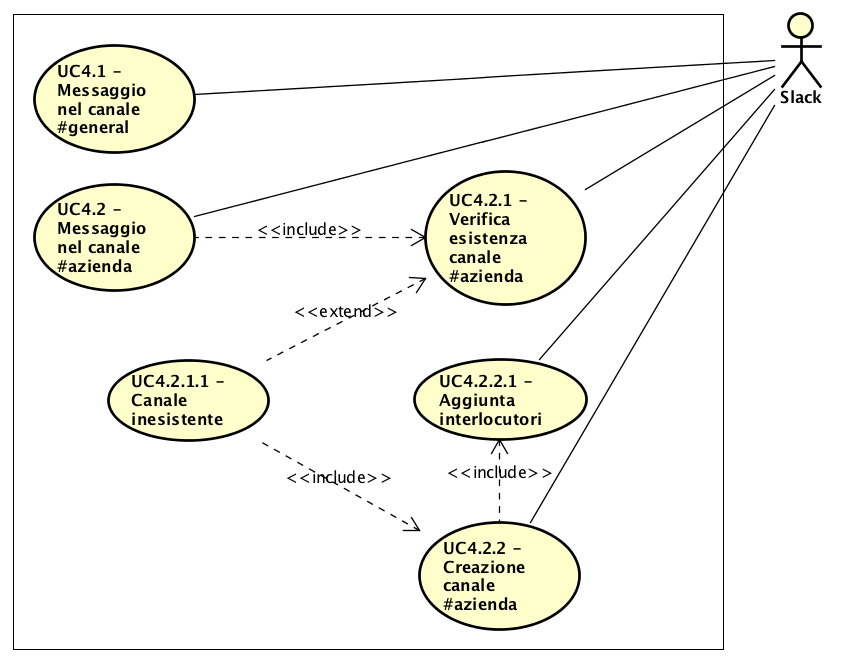
\includegraphics[width=\textwidth]{UseCases/UC4-InvioMessaggio/UC4.png}
	\caption{UC4 - Invio messaggio}
\end{figure}
\label{sssec:UC4} 
\begin{itemize} 
\item \textbf{Attori}: database, interlocutore, Slack;
\item \textbf{Descrizione}: invia un messaggio su Slack;
\item \textbf{Precondizione}: ospite autenticato;
\item \textbf{Postcondizione}: viene inviato un messaggio;
\item \textbf{Estensioni}:\begin{itemize}\item messaggio nel canale \#general (UC4.1);\item messaggio nel canale \#azienda (UC4.2).\end{itemize}
\end{itemize} 
\subsection{UC4.1 - Messaggio nel canale \#general} 
\label{sssec:UC4.1} 
\begin{itemize} 
\item \textbf{Attori}: database, Slack;
\item \textbf{Descrizione}: viene inviato un messaggio nel canale Slack \#general;
\item \textbf{Precondizione}: ho il testo del messaggio da inviare;
\item \textbf{Postcondizione}: il canale \#general riceve il messaggio;
\end{itemize} 
\subsection{UC4.2 - Messaggio nel canale \#azienda} 
\label{sssec:UC4.2} 
\begin{itemize} 
\item \textbf{Attori}: interlocutore, Slack;
\item \textbf{Descrizione}: viene inviato un messaggio nel canale corrispondente a quello dell'azienda;
\item \textbf{Precondizione}: ho il testo del messaggio ed il nome dell'azienda;
\item \textbf{Postcondizione}: il messaggio viene ricevuto nel canale;
\item \textbf{Scenario principale}: \begin{enumerate}\item verifica esistenza canale \#azienda (UC4.2.1). 
 \end{enumerate}
\item \textbf{Estensioni}:\begin{itemize}\item creazione canale \#azienda (UC4.2.2).\end{itemize}
\end{itemize} 
\subsection{UC4.2.1 - Verifica esistenza canale \#azienda} 
\label{sssec:UC4.2.1} 
\begin{itemize} 
\item \textbf{Attori}: database, Slack;
\item \textbf{Descrizione}: viene verificata l'esistenza del canale \#azienda;
\item \textbf{Precondizione}: possiedo il nome dell'azienda;
\item \textbf{Postcondizione}: ritorno l'identificativo del canale;
\item \textbf{Estensioni}:\begin{itemize}\item canale inesistente (UC4.2.1.1).\end{itemize}
\end{itemize} 
\subsection{UC4.2.1.1 - Canale inesistente} 
\label{sssec:UC4.2.1.1} 
\begin{itemize} 
\item \textbf{Attori}: Slack;
\item \textbf{Descrizione}: il canale cercato non esiste;
\item \textbf{Precondizione}: viene cercato un canale;
\item \textbf{Postcondizione}: il canale cercato non esiste;
\end{itemize} 
\subsection{UC4.2.2 - Creazione canale \#azienda} 
\label{sssec:UC4.2.2} 
\begin{itemize} 
\item \textbf{Attori}: Slack;
\item \textbf{Descrizione}: viene creato il canale per l'azienda che ancora non esiste;
\item \textbf{Precondizione}: il canale non esiste;
\item \textbf{Postcondizione}: viene creato il canale;
\item \textbf{Scenario principale}: \begin{enumerate}\item aggiunta interlocutori (UC4.2.2.1). 
 \end{enumerate}
\end{itemize} 
\subsection{UC4.2.2.1 - Aggiunta interlocutori} 
\label{sssec:UC4.2.2.1} 
\begin{itemize} 
\item \textbf{Attori}: database, interlocutore, Slack;
\item \textbf{Descrizione}: vengono aggiunti gli interlocutori nel canale \#azienda;
\item \textbf{Precondizione}: ho la lista degli interlocutori da aggiungere;
\item \textbf{Postcondizione}: vengono aggiunti gli interlocutori;
\item \textbf{Scenario principale}: chiedo alle API di Slack di aggiungere gli interlocutori.\end{itemize} 
\newpage
\subsection{UC5 - Disattivazione AV}
\begin{figure}[!h]
	\centering
	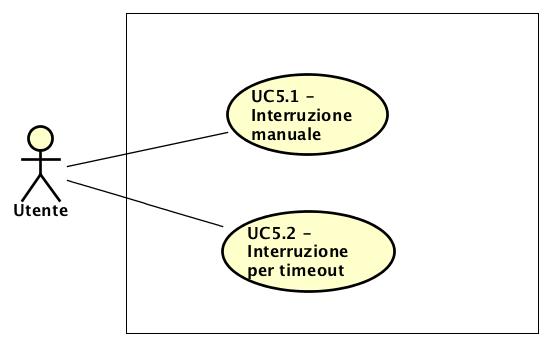
\includegraphics[width=\textwidth]{UseCases/UC5-Disattivazione/UC5.png}
	\caption{UC5 - Disattivazione AV}
\end{figure}	
\label{sssec:UC5} 
\begin{itemize} 
\item \textbf{Attori}: utente;
\item \textbf{Descrizione}: disattivazione AV;
\item \textbf{Precondizione}: ospite autenticato;
\item \textbf{Postcondizione}: l'AV è stato disattivato;
\item \textbf{Estensioni}:\begin{itemize}\item interruzione manuale (UC5.1);\item interruzione per timeout (UC5.2).\end{itemize}
\end{itemize} 
\subsection{UC5.1 - Interruzione manuale} 
\label{sssec:UC5.1} 
\begin{itemize} 
\item \textbf{Attori}: utente;
\item \textbf{Descrizione}: l'ospite/utente termina la sessione premendo sull'interfaccia Web;
\item \textbf{Precondizione}: c'è una sessione attiva;
\item \textbf{Postcondizione}: l'AV termina la sessione;
\item \textbf{Scenario principale}: viene premuto l'apposito pulsante sull'interfaccia Web e la sessione termina.\end{itemize} 
\subsection{UC5.2 - Interruzione per timeout} 
\label{sssec:UC5.2} 
\begin{itemize} 
\item \textbf{Descrizione}: la sessione termina per via della scadenza del timeout;
\item \textbf{Precondizione}: c'è una sessione attiva e l'ospite/utente non interagisce per un certo lasso di tempo prestabilito;
\item \textbf{Postcondizione}: la sessione termina;
\item \textbf{Scenario principale}: l'ospite/utente non interagisce per un certo lasso di tempo prestabilito e la sessione termina.\end{itemize} 

\newpage
\subsection{UC6 - Amministrazione} 
\begin{figure}[!h]
	\centering
	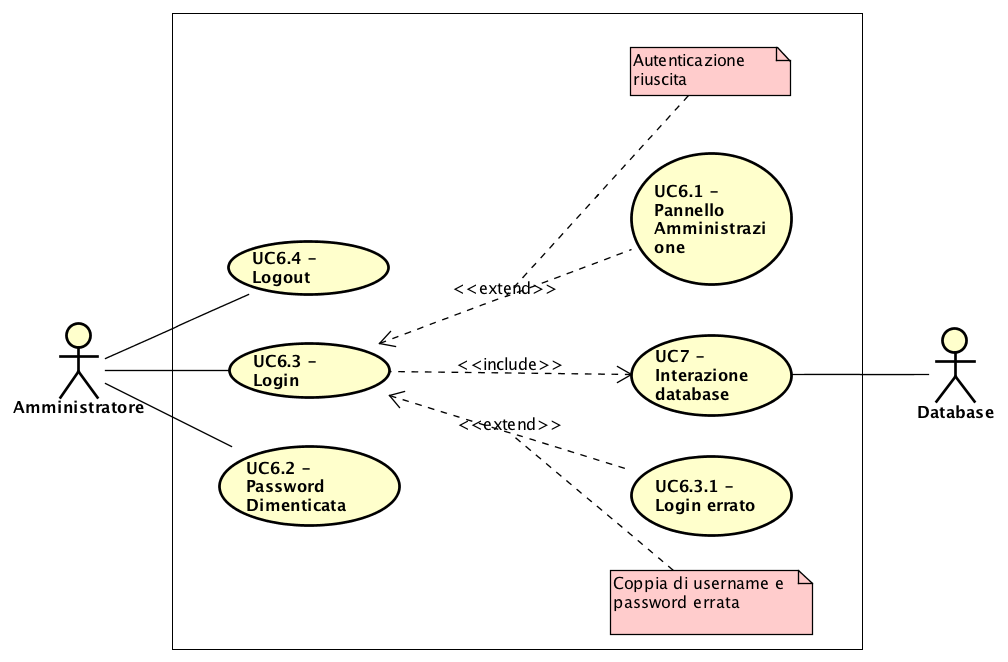
\includegraphics[width=\textwidth]{UseCases/UC6-Amministrazione/Immagini/UCPannelloAmministrazione.png}
	\caption{UC6 - Amministrazione}
\end{figure}	
\label{sssec:UC6} 
\begin{itemize} 
\item \textbf{Attori}: utente;
\item \textbf{Descrizione}: accesso a pannello di amministrazione del sistema;
\item \textbf{Precondizione}: si ha accesso alla pagina web;
\item \textbf{Postcondizione}: accesso al pannello;
\item \textbf{Estensioni}:\begin{itemize}\item pannello Amministrazione (UC6.1);\item password dimenticata (UC6.2);\item login (UC6.3);\item logout (UC6.4).\end{itemize}
\end{itemize}
\newpage
\subsection{UC6.1 - Pannello Amministrazione}
\begin{figure}[!h]
	\centering
	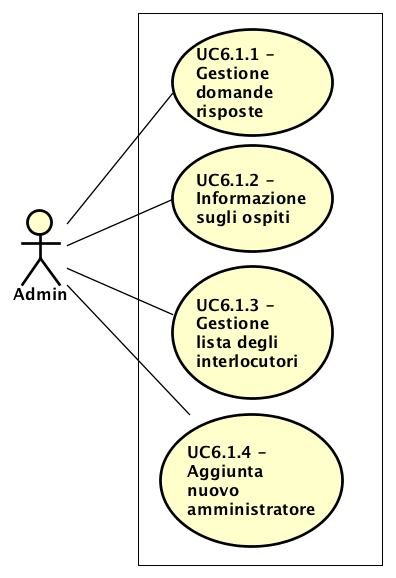
\includegraphics[scale=0.7]{UseCases/UC6-Amministrazione/Immagini/UCMenu.png}
	\caption{UC6.1 - Pannello Amministrazione}
\end{figure}	
\label{sssec:UC6.1} 
\begin{itemize} 
\item \textbf{Attori}: amministratore, database;
\item \textbf{Descrizione}: menù amministrativo di sistema;
\item \textbf{Precondizione}: l'amministratore è stato autenticato con il suo account accedendo al DB (UC7) e quindi lo possiede;
\item \textbf{Postcondizione}: l'amministratore ha scelto una delle opzioni o ha effettuato il logout;
\item \textbf{Estensioni}:\begin{itemize}\item gestione domande e risposte (UC6.1.1);\item informazioni sugli ospiti (UC6.1.2);\item gestione lista degli interlocutori (UC6.1.3);\item aggiunta nuovo amministratore (UC6.1.4).\end{itemize}
\end{itemize}
\newpage
\subsection{UC6.1.1 - Gestione domande e risposte}
\begin{figure}[!h]
	\centering
	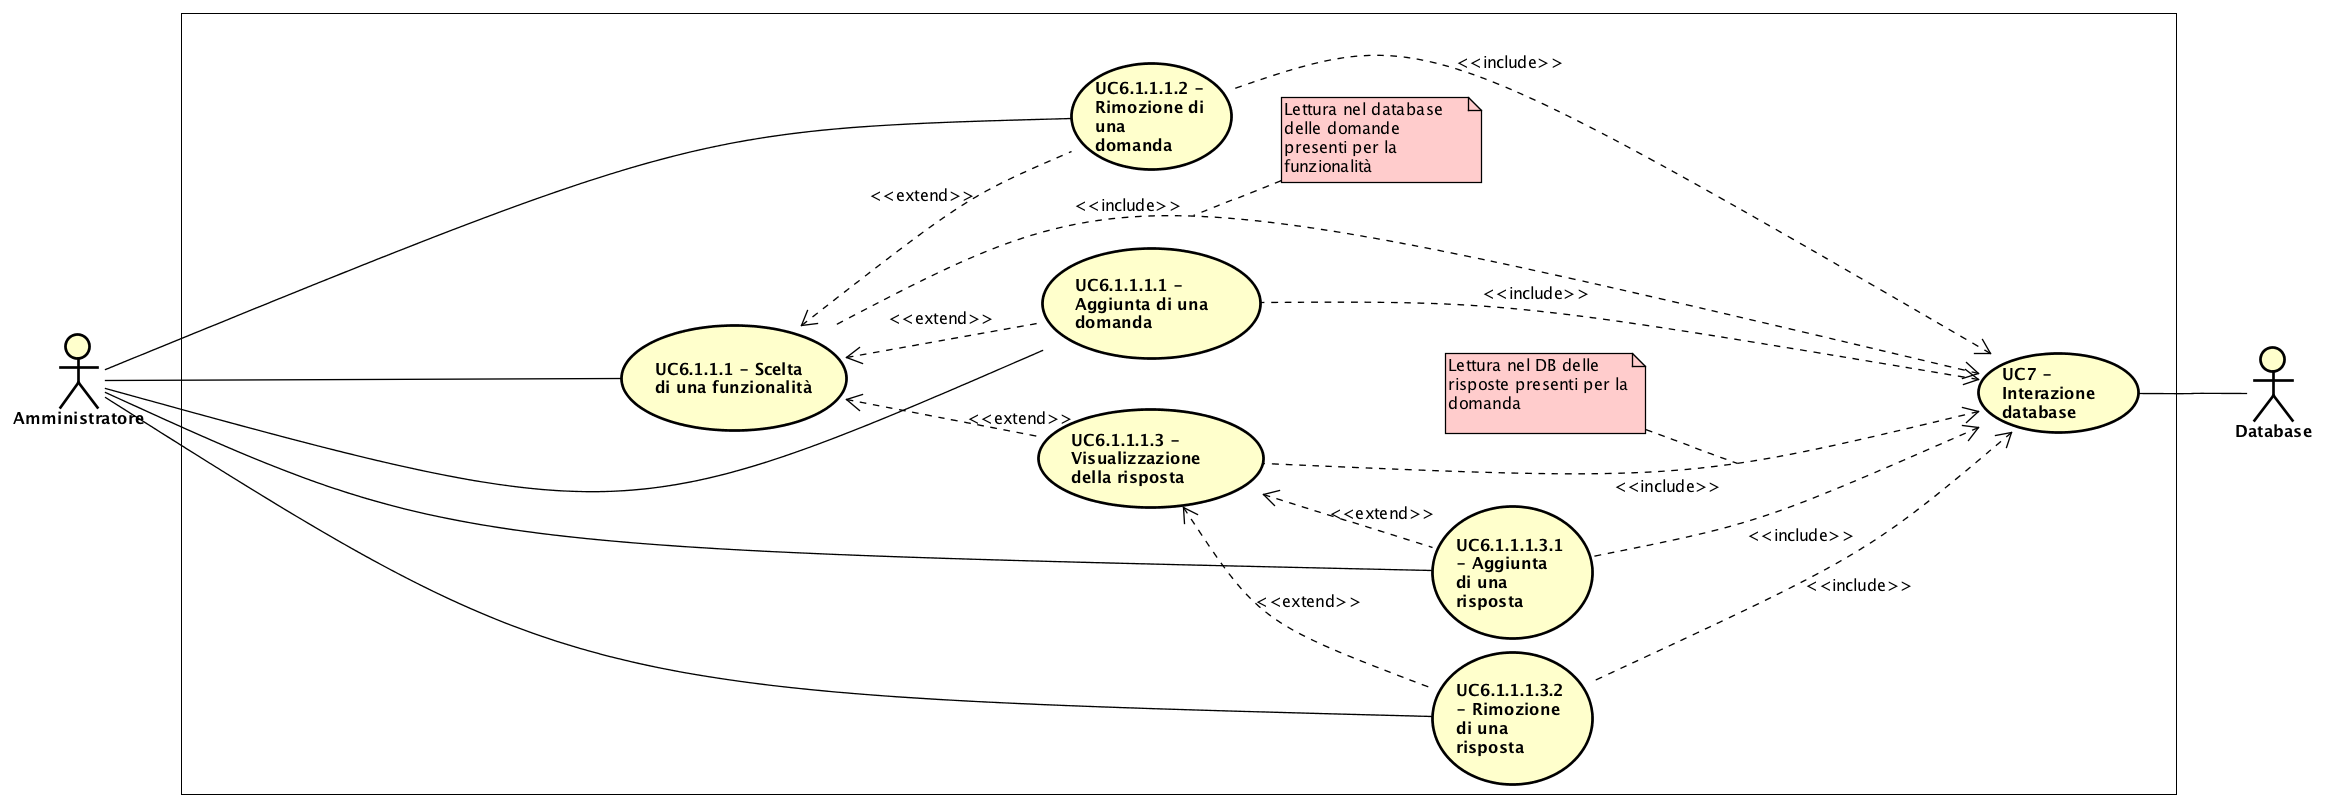
\includegraphics[width=\textwidth]{UseCases/UC6-Amministrazione/Immagini/UCGestioneDomandeERisposte.png}
	\caption{UC6.1.1 - Gestione domande e risposte}
\end{figure}	
\label{sssec:UC6.1.1} 
\begin{itemize} 
\item \textbf{Attori}: amministratore;
\item \textbf{Descrizione}: gestione delle domande e delle risposte del sistema;
\item \textbf{Precondizione}: accesso al pannello di amministrazione;
\item \textbf{Postcondizione}: accesso al pannello di gestione delle domande e delle risposte. Viene visualizzata la lista delle funzionalità delle quali si possono modificare le domande e le risposte;
\item \textbf{Scenari alternativi}: l'amministratore sceglie un altra opzione o esegue il logout.
\item \textbf{Estensioni}:\begin{itemize}\item scelta di una funzionalità (UC6.1.1.1).\end{itemize}
\end{itemize} 
\subsection{UC6.1.1.1 - Scelta di una funzionalità} 
\label{sssec:UC6.1.1.1} 
\begin{itemize} 
\item \textbf{Attori}: amministratore;
\item \textbf{Descrizione}: l'amministratore sceglie una delle funzionalità proposte dal sistema;
\item \textbf{Precondizione}: l'amministratore ha accesso al pannello di amministrazione delle domande e delle risposte;
\item \textbf{Postcondizione}: l'amministratore ha scelto una delle funzionalità;
\item \textbf{Estensioni}:\begin{itemize}\item aggiunta di una domanda (UC6.1.1.1.1);\item rimozione di una domanda (UC6.1.1.1.2);\item visualizzazione della risposta (UC6.1.1.1.3).\end{itemize}
\end{itemize} 
\subsection{UC6.1.1.1.1 - Aggiunta di una domanda} 
\label{sssec:UC6.1.1.1.1} 
\begin{itemize} 
\item \textbf{Attori}: amministratore, database;
\item \textbf{Descrizione}: menù per l'aggiunta di una domanda al sistema;
\item \textbf{Precondizione}: l'amministratore ha accesso al pannello di amministrazione delle domande e delle risposte di una funzionalità;
\item \textbf{Postcondizione}: la nuova domanda viene inserita nel DB tramite UC7;
\item \textbf{Scenario principale}: l'amministratore inserisce i dati relativi alla domanda da porre e conferma le modifiche.\end{itemize} 
\subsection{UC6.1.1.1.2 - Rimozione di una domanda} 
\label{sssec:UC6.1.1.1.2} 
\begin{itemize} 
\item \textbf{Attori}: amministratore, database;
\item \textbf{Descrizione}: rimozione di una domanda da una funzionalità;
\item \textbf{Precondizione}: l'amministratore sceglie di rimuovere una domanda;
\item \textbf{Postcondizione}: la domanda e le relative risposte vengono cancellate dal DB tramite UC7;
\item \textbf{Scenario principale}: l'amministratore sceglie una domanda da eliminare e conferma la sua intenzione.\end{itemize} 
\subsection{UC6.1.1.1.3 - Visualizzazione della risposta} 
\label{sssec:UC6.1.1.1.3} 
\begin{itemize} 
\item \textbf{Attori}: amministratore, database;
\item \textbf{Descrizione}: visualizzazione delle risposte di una delle domande;
\item \textbf{Precondizione}: accesso al pannello di amministrazione delle domande e risposte e selezione di una delle domande di una funzionalità;
\item \textbf{Postcondizione}: visualizzazione del pannello di amministrazione delle risposte di una domanda lette dal DB tramite UC7;
\item \textbf{Estensioni}:\begin{itemize}\item aggiunta di una risposta (UC6.1.1.1.3.1);\item rimozione di una risposta (UC6.1.1.1.3.2).\end{itemize}
\end{itemize} 
\subsection{UC6.1.1.1.3.1 - Aggiunta di una risposta} 
\label{sssec:UC6.1.1.1.3.1} 
\begin{itemize} 
\item \textbf{Attori}: amministratore, database;
\item \textbf{Descrizione}: aggiunta di una risposta ad una domanda;
\item \textbf{Precondizione}: accesso al pannello di amministrazione delle risposte di una domanda e inserimento di una risposta;
\item \textbf{Postcondizione}: la risposta inserita dall'amministratore viene inserita nel DB tramite UC7;
\item \textbf{Scenario principale}: l'amministratore sceglie di inserire una nuova risposta ad una domanda, inserisce la riposta in un campo di testo e conferma l'inserimento. La nuova risposta viene salvata nel DB.\end{itemize} 
\subsection{UC6.1.1.1.3.2 - Rimozione di una risposta} 
\label{sssec:UC6.1.1.1.3.2} 
\begin{itemize} 
\item \textbf{Attori}: amministratore, database;
\item \textbf{Descrizione}: rimozione di una risposta ad una domanda;
\item \textbf{Precondizione}: l'amministratore ha accesso al pannello di amministrazione delle risposte;
\item \textbf{Postcondizione}: la risposta scelta viene rimossa dal DB tramite UC7;
\item \textbf{Scenario principale}: l'amministratore sceglie una risposta da eliminare e conferma la scelta. La risposta viene rimossa dal DB.\end{itemize}
\newpage
\subsection{UC6.1.2 - Informazioni sugli ospiti}
\begin{figure}[!h]
	\centering
	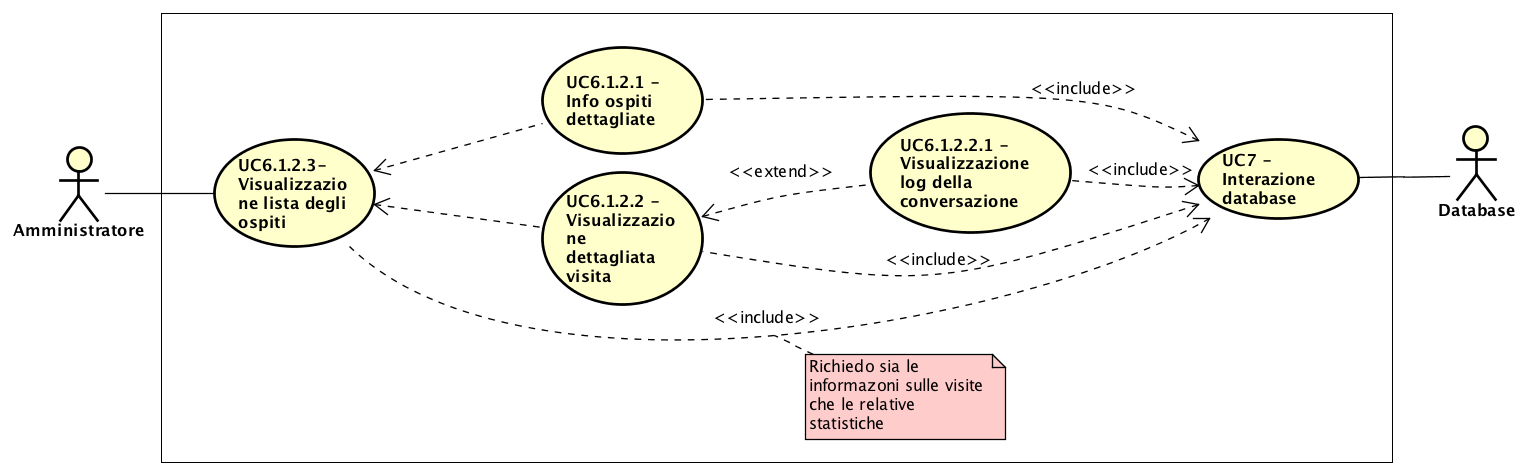
\includegraphics[width=\textwidth]{UseCases/UC6-Amministrazione/Immagini/UCInformazioniSugliOspiti.png}
	\caption{UC6.1 - Pannello Amministrazione}
\end{figure}	
\label{sssec:UC6.1.2} 
\begin{itemize} 
\item \textbf{Attori}: amministratore, database;
\item \textbf{Descrizione}: informazioni sugli ospiti che hanno interagito con l'AV;
\item \textbf{Precondizione}: accesso al pannello di amministrazione;
\item \textbf{Postcondizione}: accesso al pannello delle informazioni sugli ospiti e visualizzazione dei dati sugli ospiti del DB (UC7);
\item \textbf{Scenario principale}: \begin{enumerate}\item info ospite dettagliate (UC6.1.2.1);\item visualizzazione dettagliata visita (UC6.1.2.2);\item visualizzazione lista degli ospiti (UC6.1.2.3). 
 \end{enumerate}
\item \textbf{Scenari alternativi}: l'amministratore sceglie un altra opzione o esegue il logout.
\item \textbf{Eredi}:\begin{itemize}\item info ospite dettagliate (UC6.1.2.1)\item visualizzazione dettagliata visita (UC6.1.2.2). 
\end{itemize}\end{itemize} 
\subsection{UC6.1.2.1 - Info ospite dettagliate} 
\label{sssec:UC6.1.2.1} 
\begin{itemize} 
\item \textbf{Attori}: amministratore, database;
\item \textbf{Descrizione}: visualizzazione ulteriori informazioni sull'ospite scelto;
\item \textbf{Precondizione}: ho selezionato un ospite e ne possiedo l'identificativo;
\item \textbf{Postcondizione}: l'amministratore riceve le informazioni dell'utente;
\item \textbf{Scenario principale}: 1- l'amministratore ha cliccato su un'ospite
2- ricevo l'identificativo su un'utente e ne richiedo le informazioni al database (UC7)
3- il database ritorna le informazioni
4- le visualizzo a schermo.\end{itemize} 
\subsection{UC6.1.2.2 - Visualizzazione dettagliata visita} 
\label{sssec:UC6.1.2.2} 
\begin{itemize} 
\item \textbf{Attori}: amministratore, database;
\item \textbf{Descrizione}: visualizzazione dettagliata della visita;
\item \textbf{Precondizione}: l'amministratore ha scelto di visualizzare in dettaglio una visita di un ospite;
\item \textbf{Postcondizione}: vengono letti i dati riguardanti la visita scelta dal DB e visualizzati a schermo;
\item \textbf{Estensioni}:\begin{itemize}\item visualizzazione log della conversazione (UC6.1.2.2.1).\end{itemize}
\end{itemize} 
\subsection{UC6.1.2.2.1 - Visualizzazione log della conversazione} 
\label{sssec:UC6.1.2.2.1} 
\begin{itemize} 
\item \textbf{Attori}: amministratore, database;
\item \textbf{Descrizione}: visualizzazione del log della conversazione tra l'AV e l'ospite;
\item \textbf{Precondizione}: l'amministratore ha accesso alla pagina di visualizzazione dettagliata di una visita di un ospite;
\item \textbf{Postcondizione}: viene mostrato a schermo il log completo della conversazione con l'AV;
\item \textbf{Scenario principale}: l'amministratore sceglie di visualizzare il log della conversazione con l'AV. Vengono letti dal DB i dati richiesti. Viene mostrato a schermo il log completo.\end{itemize} 
\subsection{UC6.1.2.3 - Visualizzazione lista degli ospiti} 
\label{sssec:UC6.1.2.3} 
\begin{itemize} 
\item \textbf{Attori}: amministratore, database;
\item \textbf{Descrizione}: visualizzazione della lista degli ospiti presente nel Database;
\item \textbf{Precondizione}: l'Amministratore deve avere già effettuato il login;
\item \textbf{Postcondizione}: la lista degli ospiti viene visualizzata a video;
\item \textbf{Scenario principale}: l'Amministratore entrato nel pannello delle informazioni sugli ospiti, visualizza la lista degli ospiti che hanno effettuato una visita all'interno dell'azienda. Da questa lista ha la possibilità di ottenere informazioni più specifiche su un determinato ospite e sulle sue visite.\end{itemize}
\newpage
\subsection{UC6.1.3 - Gestione lista degli interlocutori}
\begin{figure}[!h]
	\centering
	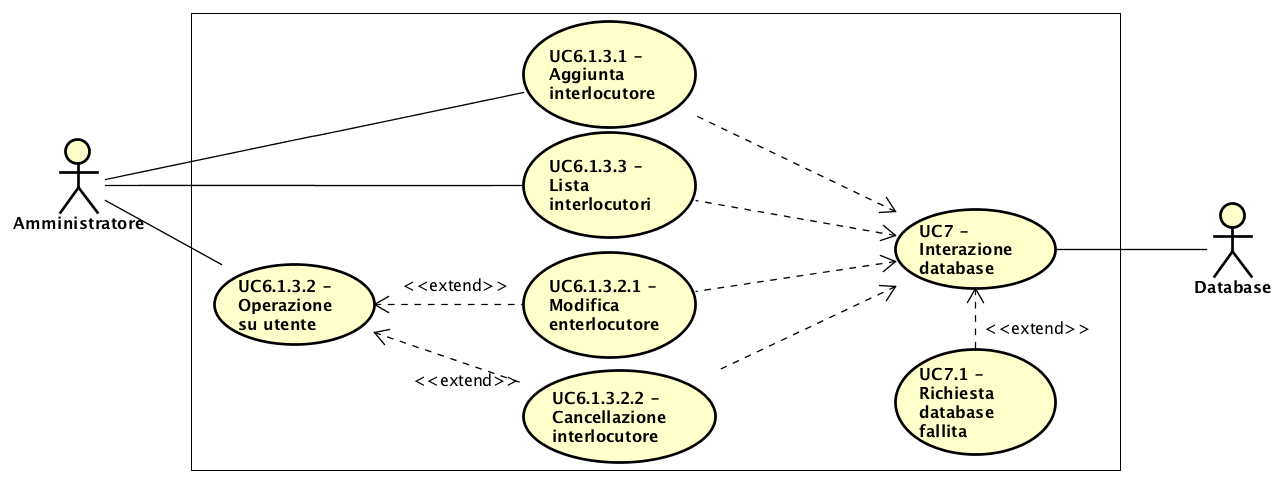
\includegraphics[width=\textwidth]{UseCases/UC6-Amministrazione/Immagini/UCGestioneListaDegliInterlocutori.png}
	\caption{UC6.1.3 - Gestione lista degli interlocutori}
\end{figure}	
\label{sssec:UC6.1.3} 
\begin{itemize} 
\item \textbf{Attori}: amministratore, database, Slack;
\item \textbf{Descrizione}: gestione degli interlocutori del sistema;
\item \textbf{Precondizione}: l'amministratore è autenticato;
\item \textbf{Postcondizione}: accesso al pannello di gestione degli interlocutori del sistema;
\item \textbf{Scenari alternativi}: l'amministratore sceglie un altra opzione o esegue il logout.
\item \textbf{Estensioni}:\begin{itemize}\item aggiunta interlocutore (UC6.1.3.1);\item operazione su utente (UC6.1.3.2);\item lista interlocutori (UC6.1.3.3).\end{itemize}
\end{itemize} 
\subsection{UC6.1.3.1 - Aggiunta interlocutore} 
\label{sssec:UC6.1.3.1} 
\begin{itemize} 
\item \textbf{Attori}: amministratore, Slack;
\item \textbf{Descrizione}: vengono controllati i dati inseriti e viene fatta la richiesta di aggiunta;
\item \textbf{Precondizione}: l'amministratore è autenticato e ha compilato i dati del nuovo interlocutore;
\item \textbf{Postcondizione}: vengono inviati i dati al database per l'inserimento;
\item \textbf{Scenario principale}: 
	\begin{enumerate}
		\item vengono compilati i dati;
		\item viene effettuata la richiesta.
	\end{enumerate} 
\end{itemize} 
\subsection{UC6.1.3.2 - Operazione su utente} 
\label{sssec:UC6.1.3.2} 
\begin{itemize} 
\item \textbf{Attori}: amministratore, database, Slack;
\item \textbf{Descrizione}: viene effettuata un'operazione su un singolo utente della lista;
\item \textbf{Precondizione}: viene visualizzata la lista degli interlocutori;
\item \textbf{Postcondizione}: si è scelto l'interlocutore da modificare;
\item \textbf{Estensioni}:\begin{itemize}\item modifica interlocutore (UC6.1.3.2.1);\item cancellazione interlocutore (UC6.1.3.2.2).\end{itemize}
\end{itemize} 
\subsection{UC6.1.3.2.1 - Modifica interlocutore} 
\label{sssec:UC6.1.3.2.1} 
\begin{itemize} 
\item \textbf{Attori}: amministratore, database, Slack;
\item \textbf{Descrizione}: vengono modificati i dati dell'interlocutore;
\item \textbf{Precondizione}: è stato selezionato un'interlocutore;
\item \textbf{Postcondizione}: l'interlocutore è stato modificato;
\item \textbf{Scenario principale}: vengono richiesti i dati dell'interlocutore al database, i dati vengono modificati e successivamente viene effettuata la richiesta di modifica al database.\end{itemize} 
\subsection{UC6.1.3.2.2 - Cancellazione interlocutore} 
\label{sssec:UC6.1.3.2.2} 
\begin{itemize} 
\item \textbf{Attori}: amministratore, database, Slack;
\item \textbf{Descrizione}: un'interlocutore viene eliminato dalla lista;
\item \textbf{Precondizione}: è stato selezionato un'utente;
\item \textbf{Postcondizione}: l'utente viene eliminato permanentemente dalla lista degli interlocutori;
\item \textbf{Scenario principale}: viene selezionato un utente da cancellare e viene fatta la richiesta di cancellazione al database.\end{itemize} 
\subsection{UC6.1.3.3 - Lista interlocutori} 
\label{sssec:UC6.1.3.3} 
\begin{itemize} 
\item \textbf{Attori}: amministratore, database, Slack;
\item \textbf{Descrizione}: visualizza la lista degli interlocutori;
\item \textbf{Precondizione}: amministratore che ha già effettuato il login;
\item \textbf{Postcondizione}: visualizzazione a video della lista degli interlocutori;
\item \textbf{Scenario principale}: viene visualizzata la lista degli interlocutori.\end{itemize} 
\subsection{UC6.1.4 - Aggiunta nuovo amministratore} 
\label{sssec:UC6.1.4} 
\begin{itemize} 
\item \textbf{Descrizione}: viene aggiunto un nuovo amministratore di sistema;
\item \textbf{Precondizione}: sono loggato come amministratore;
\item \textbf{Postcondizione}: viene creato un nuovo amministratore;
\item \textbf{Scenario principale}: vengono inseriti i dati del nuovo amministratore e viene registrato nel database.\end{itemize} 
\subsection{UC6.2 - Password dimenticata} 
\label{sssec:UC6.2} 
\begin{itemize} 
\item \textbf{Attori}: database, interlocutore, Slack, utente;
\item \textbf{Descrizione}: l'utente non ricorda la password di accesso;
\item \textbf{Precondizione}: l'utente ha accesso alla pagina web;
\item \textbf{Postcondizione}: l'utente richiede il ripristino dei propri dati di login;
\item \textbf{Scenario principale}: l'utente richiede che i propri dati vengano ripristinati, gli viene richiesto l'username e il ripristino verrà gestito tramite Slack.\end{itemize} 
\subsection{UC6.3 - Login} 
\label{sssec:UC6.3} 
\begin{itemize} 
\item \textbf{Attori}: database, utente;
\item \textbf{Descrizione}: autenticazione dell'amministratore;
\item \textbf{Precondizione}: l'amministratore non è ancora autenticato;
\item \textbf{Postcondizione}: l'amministratore è autenticato o viene sollevato un'errore;
\item \textbf{Estensioni}:\begin{itemize}\item login errato (UC6.3.1).\end{itemize}
\end{itemize} 
\subsection{UC6.3.1 - Login errato} 
\label{sssec:UC6.3.1} 
\begin{itemize} 
\item \textbf{Attori}: amministratore;
\item \textbf{Descrizione}: il login è fallito perché i dati erano errati, quindi il database non ha dato risultato positivo;
\item \textbf{Precondizione}: è stato effettuato un tentativo di login ma è fallito;
\item \textbf{Postcondizione}: viene riportato l'errore;
\item \textbf{Scenario principale}: il database ritorna al login un errore e viene riportato all'utente l'errore.\end{itemize} 
\subsection{UC6.4 - Logout} 
\label{sssec:UC6.4} 
\begin{itemize} 
\item \textbf{Attori}: utente;
\item \textbf{Descrizione}: l'amministratore viene disconnesso dal sistema e per poter riaccedere, dovrà ripetere l'autenticazione;
\item \textbf{Precondizione}: l'amministratore è autenticato;
\item \textbf{Postcondizione}: l'amministratore viene disconnesso dal sistema e per poter riaccedere, dovrà ripetere l'autenticazione;
\item \textbf{Scenario principale}: viene selezionata l'opzione logout, l'utente viene disconnesso, e riportato al login.\end{itemize} 
\newpage
\subsection{UC7 - Interazione database}
\begin{figure}[!h]
	\centering
	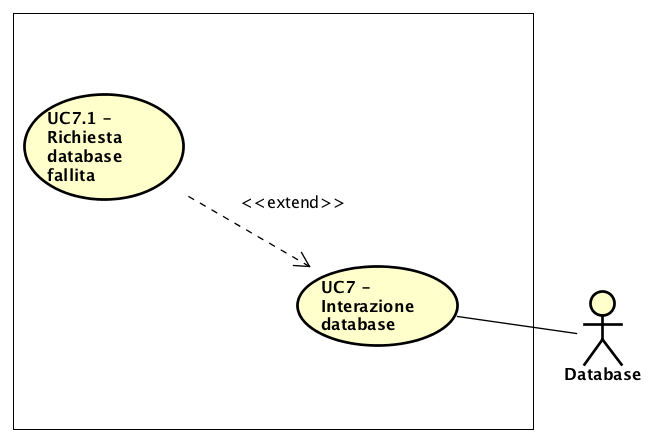
\includegraphics[width=\textwidth]{UseCases/UC7-InterazioneDB/UC7.png}
	\caption{UC7 - Interazione database}
\end{figure}
\label{sssec:UC7} 
\begin{itemize} 
\item \textbf{Attori}: database;
\item \textbf{Descrizione}: richiesta al database con relativa risposta;
\item \textbf{Precondizione}: dati di accesso al database corretti;
\item \textbf{Postcondizione}: esecuzione del comando al database e ritorno risposta o errore;
\item \textbf{Estensioni}:\begin{itemize}\item richiesta database fallita (UC7.1).\end{itemize}
\end{itemize} 
\subsection{UC7.1 - Richiesta database fallita} 
\label{sssec:UC7.1} 
\begin{itemize} 
\item \textbf{Attori}: database;
\item \textbf{Descrizione}: richiesta database fallita;
\item \textbf{Precondizione}: è stata effettuata la richiesta al database ma è fallita;
\item \textbf{Postcondizione}: viene restituito l'errore;
\item \textbf{Scenario principale}: viene effettuata la richiesta al database, ma questa fallisce, viene quindi ritornato l'errore.\end{itemize} 
\newpage
\subsection{UC8 - Interazione con Alexa}
\begin{figure}[!h]
	\centering
	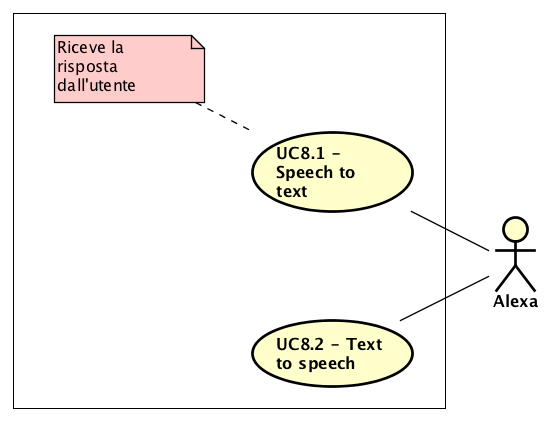
\includegraphics[width=\textwidth]{UseCases/UC8-InterazioneAlexa/UC8.png}
	\caption{UC8 - Interazione con Alexa}
\end{figure}
\label{sssec:UC8} 
\begin{itemize} 
\item \textbf{Attori}: Alexa, ospite;
\item \textbf{Descrizione}: viene richiesta un'iterazione con Alexa;
\item \textbf{Precondizione}: è stata richiesta un'interazione tra il sistema ed Alexa;
\item \textbf{Postcondizione}: ritorna il risultato di Alexa;
\item \textbf{Estensioni}:\begin{itemize}\item speech to text (UC8.1);\item text to speech (UC8.2).\end{itemize}
\end{itemize} 
\subsection{UC8.1 - Speech to text} 
\label{sssec:UC8.1} 
\begin{itemize} 
\item \textbf{Attori}: Alexa, ospite;
\item \textbf{Descrizione}: viene richiesta la traduzione da impronta vocale e testo;
\item \textbf{Precondizione}: si ha l'impronta volcale;
\item \textbf{Postcondizione}: si riceve una possibile soluzione;
\end{itemize} 
\subsection{UC8.2 - Text to speech}
\label{sssec:UC8.2} 
\begin{itemize} 
\item \textbf{Attori}: Alexa, ospite;
\item \textbf{Descrizione}: viene richiesta la traduzione da testo a impronta vocale;
\item \textbf{Precondizione}: viene proposto il testo da riprodurre;
\item \textbf{Postcondizione}: viene fornita la traccia audio;
\end{itemize} 
\newpage
\subsection{UC9 - Interazione ospite-sistema}
\begin{figure}[!h]
	\centering
	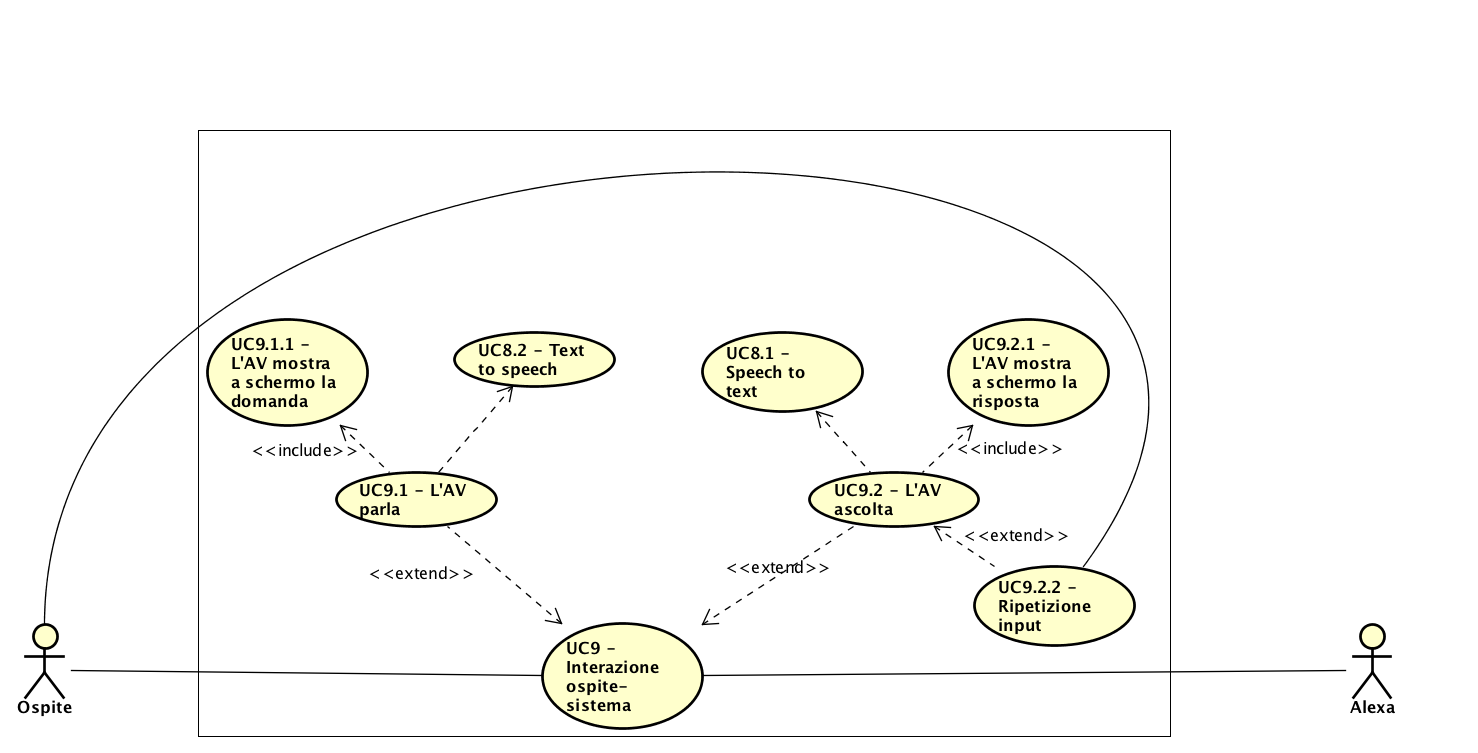
\includegraphics[width=\textwidth]{UseCases/UC9-InterazioneOspiteSistema/UC9.png}
	\caption{UC9 - Interazione ospite-sistema}
\end{figure}	
\label{sssec:UC9}
\begin{itemize} 
\item \textbf{Attori}: Alexa, ospite;
\item \textbf{Descrizione}: interazione vocale tra l'ospite di Zero12 e l'AV;
\item \textbf{Precondizione}: l'ospite può parlare, il sistema può comunicare con Alexa;
\item \textbf{Postcondizione}: l'interazione con l'ospite è avvenuta;
\item \textbf{Estensioni}:\begin{itemize}\item l'AV parla (UC9.1);\item l'AV ascolta (UC9.2).\end{itemize}
\end{itemize} 
\subsection{UC9.1 - L'AV parla} 
\label{sssec:UC9.1} 
\begin{itemize} 
\item \textbf{Attori}: Alexa, ospite;
\item \textbf{Descrizione}: l'AV pronuncia del testo all'ospite;
\item \textbf{Precondizione}: l'AV può interagire con l'utente, l'AV può interagire con Alexa, l'AV conosce cosa deve dire all'ospite;
\item \textbf{Postcondizione}: l'AV produce dei contenuti per l'ospite;
\item \textbf{Scenario principale}: \begin{enumerate}\item l'AV mostra a schermo la domanda (UC9.1.1). 
 \end{enumerate}
\end{itemize} 
\subsection{UC9.1.1 - L'AV mostra a schermo la domanda} 
\label{sssec:UC9.1.1} 
\begin{itemize} 
\item \textbf{Attori}: ospite;
\item \textbf{Descrizione}: l'AV mostra a schermo quello che ha pronunciato;
\item \textbf{Precondizione}: l'AV ha pronunciato del testo (UC9.1);
\item \textbf{Postcondizione}: sullo schermo appare il testo che l'AV ha pronunciato;
\end{itemize} 
\subsection{UC9.2 - L'AV ascolta} 
\label{sssec:UC9.2} 
\begin{itemize} 
\item \textbf{Attori}: Alexa, ospite;
\item \textbf{Descrizione}: l'AV ascolta la risposta ad una precedente interazione;
\item \textbf{Precondizione}: l'AV può interagire con Alexa, l'AV può interagire con l'ospite;
\item \textbf{Postcondizione}: l'AV riconosce la risposta;
\item \textbf{Scenario principale}: \begin{enumerate}\item l'AV mostra a schermo la risposta (UC9.2.1). 
 \end{enumerate}
\item \textbf{Estensioni}:\begin{itemize}\item ripetizione input (UC9.2.2).\end{itemize}
\end{itemize} 
\subsection{UC9.2.1 - L'AV mostra a schermo la risposta} 
\label{sssec:UC9.2.1} 
\begin{itemize} 
\item \textbf{Attori}: ospite;
\item \textbf{Descrizione}: l'AV mostra a schermo il testo che è stato compreso;
\item \textbf{Precondizione}: l'AV ha convertito l'audio della risposta in testo tramite UC8.2;
\item \textbf{Postcondizione}: l'AV mostra a schermo il testo dell'audio convertito;
\end{itemize} 
\subsection{UC9.2.2 - Ripetizione input} 
\label{sssec:UC9.2.2} 
\begin{itemize} 
\item \textbf{Attori}: ospite;
\item \textbf{Descrizione}: l'AV permette all'ospite di ripetere la propria risposta;
\item \textbf{Precondizione}: l'AV ascolta la risposta dell'ospite;
\item \textbf{Postcondizione}: l'AV ripete l'ascolto da capo;
\item \textbf{Scenario principale}: l'ospite, leggendo su schermo quello che l'AV ha compreso della sua pronuncia, si accorge di un errore, preme un pulsante a schermo per ripetere l'inserimento e l'AV ricomincia ad ascoltare la risposta dell'ospite da capo.\end{itemize} 

\end{document}